\Chapter{Témaköri áttekintés}

\section{Hasonló célú szoftverek}
\subsection{Road Traffic Library}


Az eddigi közlekedés-szimuláló szoftverek közül kiemelném először az AnyLogic által készített Road Traffic Library-t. Ezen szoftver segítségével létre lehet hozni egy úthálózatot
különböző elemekből, mint például egyenes, kanyar, útkereszteződés, híd, zebra, lámpás útkereszteződés, valamint buszmegállók és parkolók.
A szoftver képes különböző közlekedési szabályok alkalmazására, valamint a járművek intelligens módon választják meg a haladáshoz szükséges útvonalat.
Valós-idejű szimuláció futtatására is van lehetőség, 2D-ben és 3D-ben is. 

\begin{figure}[h]
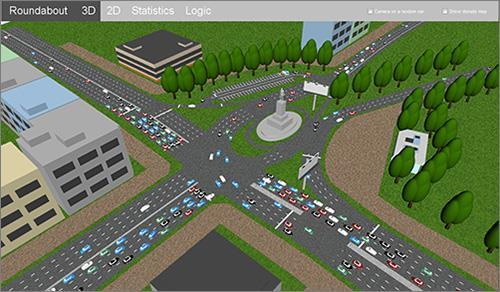
\includegraphics[width=\linewidth]{RTL.png}
\caption{Kép a Road Traffic Library-ből}
\label{fig:RTL}
\end{figure}

A szimulációkat felhasználva hőtérkép is előállítható, amely megmutatja mennyire voltak
forgalmasak az adott területek, így egyértelművé válik hol alakul ki könnyedén forgalmi dugó.

Lehetőség van a geoinformációs rendszerekben használt vektorgrafikus formátum, azaz shapefile importálására is. Ezen fájl alapján a szoftver automatikusan
előállítja az úthálózatot. A szoftver bővíthető még gyalogos- és vasútforgalomra vonatkozó könyvtárakkal is.

A gyalogos könyvtár segítségével szimulálható a gyalogosforgalom sűrűsége különböző környezetekben. Ilyen környezet lehet például egy buszmegálló, vagy vasútállomás területe. Az egyes épületek
felépítése is befolyásolja a forgalom sűrűségét, a gyalogosok minden akadályt, ebbe beleértve egymást is, próbálnak elkerülni.

A vasút könyvtár segítségével egy pályaudvar vasútforgalma komplex módon szimulálható. A forgalmat befolyásolja a tehervonatok rakodási ideje, a karbantartás, üzleti folyamatok lefolyása, és sok
más további esemény is.
\subsection{SUMO}

A SUMO, azaz Simulation of Urban MObility egy ingyenes, nyílt, közlekedés-szimuláló C++-ban írt szoftver. Az első verzió 2001-ben került kiadásra, azóta már az 1.1.0-ás verziószámnál jár. Ez a szoftver lehetőséget ad több közlekedési forma (tömegközlekedés, gyalogosok, stb)
modelezzésére a személygépjárművek mellett. Továbbá nagy eszköztárral bír az olyanokhoz mint útvonaltervezés, káros-anyag kibocsátás, valamint vizuális megjelenítés.
Lehetséges továbbá meglévő úthálózat importálása fájlból, valamint személyre szabott modellek használata. A SUMO nem tartalmaz semmilyen megkötést az úthálózat méretét, vagy az egyszerre szimulálható járművek számát illetően.
\begin{figure}[h]
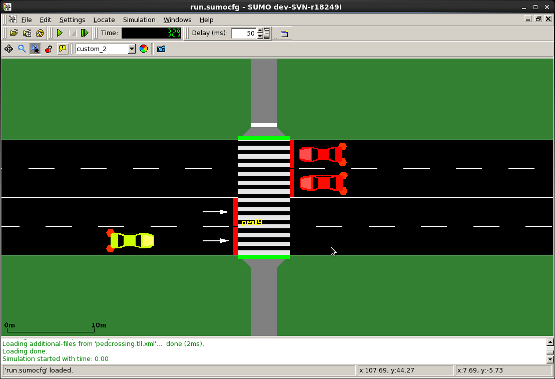
\includegraphics[width=\linewidth]{SUMO.png}
\caption{Kép a SUMO programból}
\label{fig:SUMO}
\end{figure}

A program lehetőséget ad a szimuláció online történő kezelésére is, a TraCI, azaz Traffic Control Interface használatával. Ilyen esetben a SUMO tulajdonképpen egy szerver, amelyet
egy vagy több kliensen keresztül tudunk vezérelni. TCP alapú kliens/szerver architektúrát használ. 

A közlekedési lámpák viselkedését egyénileg be lehet állítani, vagy akár előre
megírt TLS programból is lehetséges importálni. Az importáláshoz számos python szkript áll rendelkezésre. Ha nem áll rendelkezésre TLS program, a SUMO képes automatikusan generálni
egyet. Ilyenkor alapértelmezett értékeket rendel minden paraméterhez amelynek értéke nem volt kapcsolókkal definiálva. Ezek közé tartoznak:
\begin{itemize}
\item --tls.cycle.time - lámpák váltási ideje.
\item --tls.yellow.time - mennyi időre sárga a lámpa, ez alapértelmezetten az utak sebességhatára alapján történik kiszámításra.
\item --tls.minor-left.max-speed - az útkereszteződésben balra kanyarodást megengedő sebességhatár (ha az út sebességhatára ezen érték felé esik, nem engedélyezett a balra kanyarodás.)
\item --tls.left-green.time - ha egyszerre kap zöldet az egyenesen haladó, és a vele szemből balra kanyarodó, ezen érték idejéig a balra kanyarodó kap elsőbbséget.
\item --tls.allred.time - minden zöld lámpa előtt ezen értéknek megfelelő ideig piros az összes lámpa (alapértelmezetten 0.)
\item --tls.default-type - actuated értékre állítva változó hosszúságú ideig tartanak a zöld lámpák.
\end{itemize}

A szoftver alkalmas a közlekedési lámpák teljesítményének vizsgálatára, olyan útvonal-tervezésre amely igyekszik a káros-anyag kibocsátást és a légszennyezést
minimalizálni. A gyakorlatban történt híresebb alkalmazásai tartozik például a 2006-os labdarúgó világbajnokság-, valamint a Pápa 2005-ös Kölni látogatása során a közlekedés előrejelzése.

Maga a programcsomag tartalmazza a parancssori SUMO szoftvert, a grafikus felülettel ellátott GUISIM-et, egy úthálózat importáló NETCONVERT szoftvert, úthálózat generáló NETGEN szoftvert, 
egy OD2TRIPS nevű alkalmazást amely O/D mátrix alapján generál útvonalat, számos útvonal generátort, valamint egy grafikus úthálózat-szerkesztő alkalmazást.
\section{Meglévő térkép-adatbázisok modellje}

A Google Maps az egyik legelterjedtebb úthálózat-vizualizálásra alkalmas szoftver. Ez egy JavaScript alapú webalkalmazás, mely a geoinformációs adatok megjelenítése
mellett valós-idejű forgalom elemzésre is képes. 

Ehhez az adatokat több féle forrásból állítják elő. A Base Map program keretében rengeteg különböző forrásból
szereztek vektoradatokat a létező úthálózatokról. Később ennek a nevét Geo Data Upload-ra váltották, viszont a lényege ugyan az maradt.
Továbbá szereznek adatokat műholdképekből, Android rendszerű okostelefonok szolgáltatásai által, valamint a nemrég bevezetett "Helyi Idegenvezetők" funkcióval, amin keresztül
bárki tölthet fel adatokat. 

A valós-idejű forgalomelemzéshez kezdetekben a helyi önkormányzatok által szolgáltatott adatokat használták, melyeket az egyes helyeken felszerelt
szenzorok segítségével gyűjtöttek be. Viszont ezek csak a legforgalmasabb utakról adtak információt, ezért később áttértek a "crowd-source" módszerhez. Ezzel a módszerrel egy
Google Maps-et futtató okostelefon GPS adatait felhasználva ad becslést egy út forgalmasságára. Lényegében azt elemzi, mennyien küldtek GPS adatot egy adott útszakaszon azonos időben.

Az utak és más objektumok kirajzolásához a böngésző leegyszerűsített vektoradatokat kap, melyek alapján felépíti az azoknak megfelelő formákat.
Minden egyes objektumhoz tartoznak különböző metaadatok, mint például a sebességkorlát, haladási irány, út típusa (főút, stb), valamint egy név. Az objektumok JSON formában vannak
tárolva, maga a Google Maps API pedig támogatja a GeoJSON forrásból történő adatok betöltését térképekre.
Ezen információk alapján épül fel a modell amit a böngésző 2D vagy 3D formában ábrázol egy térképen.
\section{GeoSpatial adatbázisok}

A GeoSpatial adatbázisok adják az előbbi szolgáltatások hátterét. Ezek az adatbázisok kifejezetten a térbeli objektumokat leíró adatok tárolására, azok egyszerű lekérdezésére
vannak optimalizálva. A leggyakoribb adatok pontok, vonalak, vagy poligonok formájában fordulnak elő. 

A hagyományos adatbázisokhoz képest sokkal nagyobb teljesítményt nyújtanak
ilyen területen, valamint gyakran az ilyen típusú adatok feldolgozásához bővíteni kell azok funkcionalitását. Ennek érdekében az Open Geospatial Consortium 1997-től kezdődően
definiálta az ISO 19125 szabványt ezen funckionalitás megvalósításához, melynek második része leírja az SQL-ben történő megvalósítást is. Az OpenGIS szabvány ugyan magába
foglalja a CORBA és az OLE/COM implementációkat is, ezek nem részei az ISO szabványnak.

A szabvány többek között a következő műveleteket definiálja:
\begin{itemize}
\item Térbeli számítások, azaz objektumok közti távolság, vonalak hossza, stb
\item Térbeli predikátumok, objektumok közötti kapcsolatokat leíró logikai lekérdezések
\item Geometriai konstruktorok, alakzatot leíró adatok alapján új geometriai elem létrehozása
\item Egy tetszőleges objektumhoz tartozó információk lekérdezése
\end{itemize}

